\section{Phased broadband spectra from single chirp excitation}
\label{sec:bbqchili}

The are numerous nuclei of considerable interest to \ac{NMR} practitioners with
very wide chemical shift ranges, including \textsuperscript{13}C,
\textsuperscript{19}F, which is of particular interest in the pharmaceutical
industry, and \textsuperscript{31}P. Attaining spectra covering the entire
chemical shift range of such spins for use in quantitative applications is
challenging due to off-resonance effects severely effecting the amplitude and
phase of resonances with frequencies far from the transmitter
frequency\cite[Section 3.4.1]{Cavanagh2007}. One popular means of achieving
broadband excitation is to use swept-frequency (chirp)
pulses\cite{Bohlen1989,Bohlen1993}, whose frequency varies linearly with time.
The application of a single \ang{90} chirp pulse to achieve broadband
excitation, while simple, yields spectra with undesirable quadratic phase
variation with resonance frequency, on account of resonance with different
frequencies being excited at different moments in time. However, with
appropriate post-processing, it is possible to recover well-phased broadband
spectra from such datasets. In this section, a description of a method given
the name \ac{BBQCHILI} is presented, which estimates the parameters associated
with a single chirp excitation dataset, and subsequently generates a spectrum
devoid of the undesirable phase behaviour.

\subsection{An overview of single chirp excitation}
In this work, a pulse sequence comprising a single chirp pulse of duration
$\tau_{\text{p}}$, followed by a pre-scan delay of duration $\tau_{\text{del}}$
before acquisition is considered (Figure \ref{fig:single-chirp}).
Focus is limited to chirp pulses which linearly sweep frequencies
with a bandwidth $\Updelta F$, such that for a pulse of length
$\tau_{\text{p}}$, the rate at which the frequency is increased (the sweep
rate) is $\nicefrac{\Updelta F}{\tau_{\text{p}}}$. The frequencies that the
pulse sweeps through are in the range $[\foffone - \nicefrac{\Updelta F}{2},
\foffone + \nicefrac{\Updelta F}{2}]$. The \ac{RF} amplitude $\nu_{\text{RF}}$
(\unit{\hertz}) of the pulse is given by
\begin{equation}
    \nu_{\text{RF}} = \sqrt{
        \frac{\Updelta F Q}{2 \pi \tau_{\text{p}}}
    },
\end{equation}
where $Q$ is the adiabaticity factor \note{More detail/citation?}. For a pulse
with flip angle  $\beta < \ang{180}$,  $Q$ is related to $\beta$ via
\begin{equation}
    Q = \frac{2}{\pi} \ln \left( \frac{2}{\cos(\beta) + 1} \right),
\end{equation}
such that an appropriate pulse to achieve a flip angle of \ang{90} requires
selecting a combination of $\nu_{\text{RF}}$, $\Updelta F$, and
$\tau_{\text{p}}$ which satisfies $Q \approx 0.441$.

\begin{figure}
    \centering
    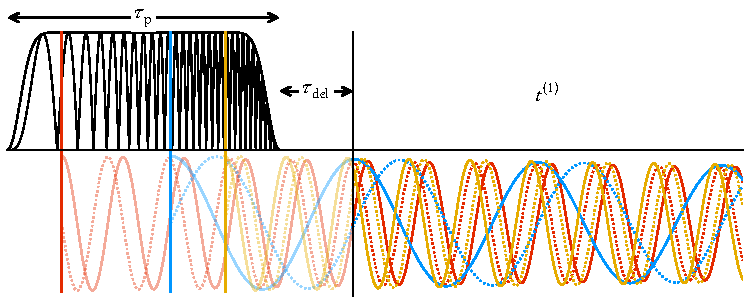
\includegraphics{single_chirp_illustration/single_chirp_illustration.pdf}
    \caption{
        An illustration of an experiment comprising a single chirp pulse sweeping
        low to high frequencies of duration $\tau_{\text{p}}$, followed by
        a pre-scan delay period or $\tau_{\text{del}}$, prior to
        acquisition. The fate of three resonances with different frequencies is
        denoted, with $\fone_{\text{red}} < \fone_{\text{blue}} <
        \fone_{\text{yellow}}$. Each resonance is excited at different points
        in time, with lower frequency resonances being excited earlier, such that
        each resonance is allowed to evolve in the transverse plane for
        different amounts of time prior to acquisition.
        The resulting \ac{FID} possesses quadratic phase behaviour.
        Coloured oscillations denote the evolution of each resonance with time,
        with solid and dashed lines representing the real and imaginary
        components of the quadrature data, respectively. The oscillations are
        paler prior to the start of acquisition.
    }
    \label{fig:single-chirp}
\end{figure}

Assuming that the chirp pulse induces an instantaneous \ang{90} rotation of a
spin at the point of resonance, the quadratic phase behaviour of the \ac{FT} of
the \ac{FID} can be corrected using phase correction (Section
\ref{subsec:nmr-analysis}), with
\begin{equation}
    \phi \left( \fone \right) = \phi_0 + 2 \pi \left(\fone - \foffone\right) \left(\tau_{\text{del}}
    + \frac{\tau_{\text{p}}}{2} \right) -
    2 \pi \left(\fone - \foffone\right)^2 \left( \frac{\tau_{\text{p}}}{2
    \Updelta F} \right)
    \label{eq:quadratic-phase}
\end{equation}
The first- and second-order phase can be dealt with using knowledge of the
pulse sequence parameters, leaving a trivial zero-order phase correction to be
determined (i.e. determination of $\phi_0$).

While \eqref{eq:quadratic-phase} is able to correct the quadratic phase
behaviour of peaks, it is unable to address another issue with the dataset,
which is the fact that for each resonance, a number of initial points are not
present in the \ac{FID}. This is illustrated by the faded sections of the
oscillators is Figure \ref{fig:single-chirp}, which no not contribute to the
\ac{FID} as acquisition is yet to start. For any resonance, the signal that is
actually detected can be thought of as the difference between two signals: (a)
the ``complete'' signal, which starts at the time of excitation, and (b)
a ``truncated'' signal which is identical to the complete signal before
acquisition, and which comprises zeros once acquisition has begun. The
linear nature of the \ac{FT} dictates that the resulting delayed-acquisition
spectrum comprises the difference between the \acp{FT} the complete signal and
the truncated signal.  The \ac{FT} of the truncated \ac{FID} is well
approximated as a broad sinc
wiggle with its maximum at the resonance frequency. The form of the wiggle
depends on the delay between excitation and acquisition, with resonances of
lower frequencies, which more of the signal is missed, displaying deeper, and
narrower artefacts (panel b of Figure \ref{fig:chirp-phase-vs-backprop}).

Both quadratic phase and missing-point artefacts can be resolved if an estimate
of the \acp{FID} parameters is obtained, as each oscillator can be
back-propagated by the requisite amount such that is begins at the point of
excitation. For an oscillator determined to have a frequency of $\fone$, the
oscillator is back-propagated such that it begins at time $t_0$, given by
\begin{equation}
    t_0\left( \fone \right) =
        -\left(\tau_{\text{del}} + \frac{\tau_{\text{p}}}{2} -
        \frac{\left( \fone - \foffone \right) \tau_{\text{p}}}{2 \Updelta F}
    \right).
\end{equation}
\begin{subequations}
    \begin{gather}
        \by_{\text{corr}} \left[ \none \right] =
            \sum_{m=0}^{M-1} \bdam \exp \left( \iu \bdphim \right)
            \exp\left(
                \left( 2 \pi \iu \bdfonem - \bdetaone \right)
                t_0 \left(\bdfonem\right) \none \Dtone
                \right)
    \end{gather}
\end{subequations}

\begin{figure}
    \centering
    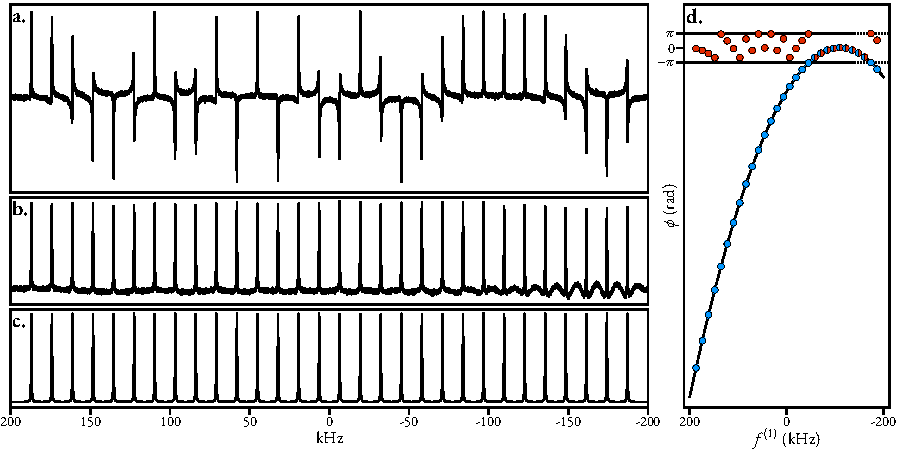
\includegraphics{chirp_phase_vs_estimation/chirp_phase_vs_estimation.pdf}
    \caption{
        Comparison of quadratic phase correction vs frequency-dependent
        back-propagation in treating data derived from a simulation of a
        single-chirp excitation experiment for a sample of 30 uniformly spaced
        isolated spins.
        \textbf{a.} Unprocessed spectrum, displaying quadratic phase behaviour.
        \textbf{b.} Spectrum generated using quadratic phase correction, with
        \eqref{eq:quadratic-phase}.
        \textbf{c.} Spectrum generated from estimation using the \ac{MPM}, and
        back-propagation.
    }
    \label{fig:chirp-phase-vs-backprop}
\end{figure}
